\documentclass[10pt,a4paper]{article}

\newcommand{\DocumentTitle}{Security Self-Assessment}

\usepackage[a4paper,left=17mm,right=17mm,top=26mm,bottom=21mm,headheight=20pt,headsep=10mm]{geometry}
\usepackage{fix-cm}
\usepackage{fontspec}
\setmainfont{texgyreheros-regular.otf}[BoldFont=texgyreheros-bold.otf,ItalicFont=texgyreheros-italic.otf]
\setmonofont{lmmono10-regular.otf}
\usepackage[table]{xcolor}
\usepackage{array,booktabs,ragged2e}
\newcolumntype{L}[1]{>{\raggedright\arraybackslash}p{\dimexpr #1\linewidth-2\tabcolsep\relax}}
\usepackage{amsmath}
\usepackage{tikz}
\usetikzlibrary{arrows.meta,positioning}
\usepackage{fancyhdr,lastpage}
\usepackage{fancyvrb}
\usepackage{titlesec}
\usepackage{hyperref}
\definecolor{Navy}{HTML}{112744}
\definecolor{Blue}{HTML}{2463AD}
\definecolor{Ink}{HTML}{23354C}
\definecolor{Muted}{HTML}{586A80}
\definecolor{Pale}{HTML}{EDF4FC}
\definecolor{Stripe}{HTML}{F5F8FC}
\definecolor{Border}{HTML}{DCE5EF}
\definecolor{Amber}{HTML}{FFF5E4}
\hypersetup{colorlinks=true,urlcolor=Blue,linkcolor=Blue,pdftitle={BizWizard - \DocumentTitle},pdfauthor={BizWizard project}}
\pagestyle{fancy}
\fancyhf{}
\fancyhead[L]{\textcolor{Blue}{\bfseries BW}\quad\textcolor{Navy}{\bfseries BizWizard}}
\fancyhead[R]{\footnotesize\textcolor{Muted}{\DocumentTitle\ | Topic E}}
\fancyfoot[L]{\scriptsize\textcolor{Muted}{BizWizard | \DocumentTitle}}
\fancyfoot[R]{\scriptsize\textcolor{Muted}{\thepage\ / \pageref*{LastPage}}}
\renewcommand{\headrulewidth}{0pt}
\renewcommand{\footrulewidth}{0.3pt}
\renewcommand{\footrule}{\hbox to\headwidth{\color{Border}\leaders\hrule height \footrulewidth\hfill}}
\setlength{\parindent}{0pt}
\setlength{\parskip}{6pt}
\setlength{\emergencystretch}{2em}
\raggedbottom
\AtBeginDocument{\fontsize{10}{14}\selectfont\color{Ink}\raggedright}
\titleformat{\subsection}{\color{Navy}\bfseries\fontsize{12}{16}\selectfont}{}{0pt}{}
\titlespacing*{\subsection}{0pt}{9pt}{4pt}
\newcommand{\DocSection}[3]{%
  {\color{Blue}\bfseries\fontsize{9}{12}\selectfont #1\par}\vspace{5pt}%
  {\color{Navy}\bfseries\fontsize{24}{28}\selectfont #2\par}\vspace{3pt}%
  {\color{Muted}\fontsize{10.5}{15}\selectfont #3\par}\vspace{6pt}}
\newcommand{\SmallText}[1]{{\color{Muted}\fontsize{8.5}{11.5}\selectfont #1\par}}
\newcommand{\EvidenceFile}[1]{\href{https://github.com/mahfuz-saim/bizwizard/blob/main/evidence/submission/#1}{\nolinkurl{#1}}}
\newcommand{\EvidenceRevision}{\SmallText{Recorded on 18 October 2026 (UTC), from clean revision \texttt{8f394d2d074b}. These are saved results, not a fresh test of the current release. Each JSON report includes the full revision and source hashes.}}
\newcommand{\DocNote}[2][Pale]{%
  \par\begingroup\setlength{\fboxsep}{9pt}%
  \colorbox{#1}{\parbox{\dimexpr\linewidth-18pt\relax}{\raggedright #2}}\endgroup\par}
\newenvironment{ReportTable}[1]{%
  \par\begingroup\fontsize{9.2}{12.5}\selectfont%
  \setlength{\tabcolsep}{6pt}\setlength{\extrarowheight}{4pt}%
  \renewcommand{\arraystretch}{1.12}%
  \rowcolors{2}{white}{Stripe}\begin{tabular}{#1}}
  {\end{tabular}\endgroup\par}
\DefineVerbatimEnvironment{CodeBlock}{Verbatim}{fontsize=\footnotesize,frame=single,framerule=0.4pt,framesep=8pt,rulecolor=\color{Border},xleftmargin=0pt,xrightmargin=0pt}
\tikzset{docbox/.style={draw=Border,fill=Pale,rounded corners=4pt,align=left,inner sep=8pt,text width=0.265\linewidth,font=\fontsize{8.5}{11.5}\selectfont},flow/.style={-{Stealth[length=4pt]},draw=Blue,line width=0.8pt}}
\newcommand{\ArchitectureDiagram}{%
\begin{center}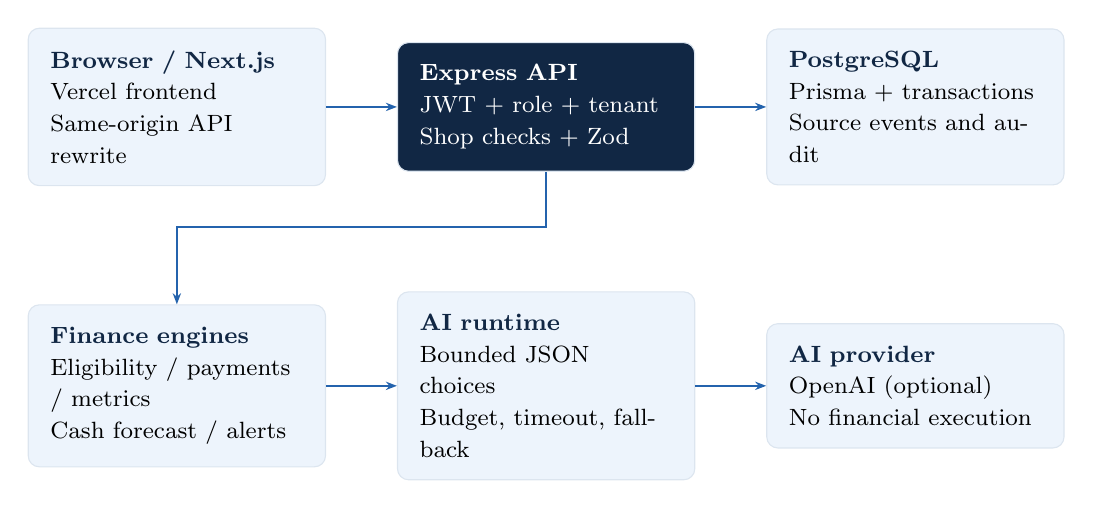
\begin{tikzpicture}[node distance=15mm and 9mm]
  \node[docbox] (browser) {\textcolor{Navy}{\bfseries Browser / Next.js}\\Vercel frontend\\Same-origin API rewrite};
  \node[docbox,right=of browser,fill=Navy,text=white] (api) {\bfseries Express API\normalfont\\JWT + role + tenant\\Shop checks + Zod};
  \node[docbox,right=of api] (db) {\textcolor{Navy}{\bfseries PostgreSQL}\\Prisma + transactions\\Source events and audit};
  \node[docbox,below=of browser] (rules) {\textcolor{Navy}{\bfseries Finance engines}\\Eligibility / payments / metrics\\Cash forecast / alerts};
  \node[docbox,right=of rules] (ai) {\textcolor{Navy}{\bfseries AI runtime}\\Bounded JSON choices\\Budget, timeout, fallback};
  \node[docbox,right=of ai] (external) {\textcolor{Navy}{\bfseries AI provider}\\OpenAI (optional)\\No financial execution};
  \draw[flow] (browser)--(api);\draw[flow] (api)--(db);
  \draw[flow] (api.south)--++(0,-7mm)-|(rules.north);
  \draw[flow] (rules)--(ai);\draw[flow] (ai)--(external);
\end{tikzpicture}\end{center}
\SmallText{Trust boundaries: browser | application/VPS | database | optional external providers}}
\newcommand{\EvaluationDiagram}{%
\begin{center}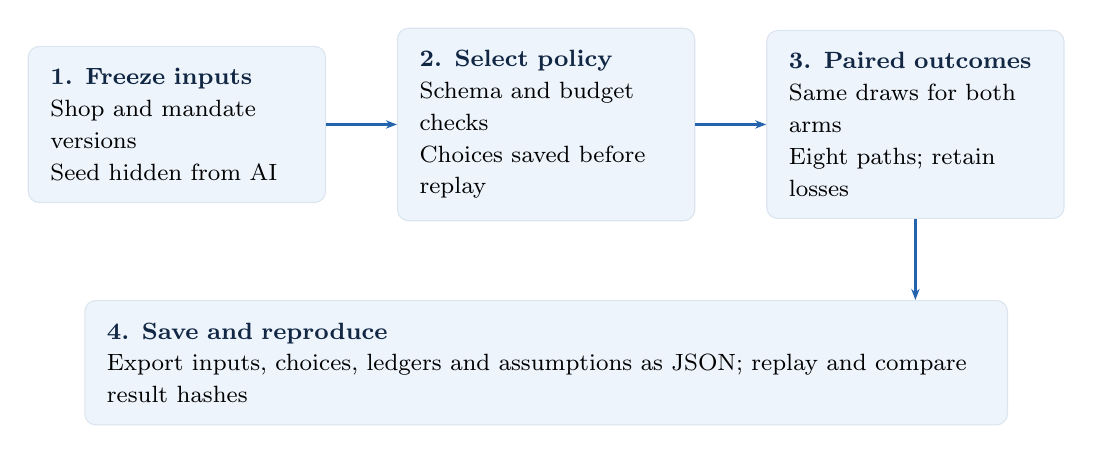
\begin{tikzpicture}[node distance=9mm]
  \node[docbox] (inputs) {\textcolor{Navy}{\bfseries 1. Freeze inputs}\\Shop and mandate versions\\Seed hidden from AI};
  \node[docbox,right=of inputs] (choices) {\textcolor{Navy}{\bfseries 2. Select policy}\\Schema and budget checks\\Choices saved before replay};
  \node[docbox,right=of choices] (outcomes) {\textcolor{Navy}{\bfseries 3. Paired outcomes}\\Same draws for both arms\\Eight paths; retain losses};
  \node[docbox,below=10mm of choices,text width=0.92\linewidth] (export) {\textcolor{Navy}{\bfseries 4. Save and reproduce}\\Export inputs, choices, ledgers and assumptions as JSON; replay and compare result hashes};
  \draw[flow] (inputs)--(choices);\draw[flow] (choices)--(outcomes);\draw[flow] (outcomes.south)--(outcomes.south |- export.north);
\end{tikzpicture}\end{center}}


\begin{document}

\DocSection{01 / ASSESSMENT OVERVIEW}{Security Self-Assessment}{2026 FinTechathon International Track\newline Topic E - SME Finance Copilot}

\DocNote{\textbf{Assessment method:} implementation review and reproducible tests in an isolated environment. Independent penetration testing and regulatory certification are outside the scope of this assessment.}

\subsection*{Scope and protected assets}

BizWizard combines daily business management with a finance copilot using the platform's saved records. This assessment focuses on the finance APIs: sign-in checks, business/shop separation, owner approvals, AI validation, cost controls, audit records and simulator isolation. It is not a security review of every business-management module.

Protected assets include sales, debts, expenses, stock, cash balances, policy versions, repayment schedules, sign-in tokens, provider credentials and financial exports. A tenant is a business account; it may contain multiple shops.


\begin{ReportTable}{L{0.247505}L{0.752495}}

\rowcolor{Navy} \textcolor{white}{\textbf{Trust zone}} & \textcolor{white}{\textbf{Security assumption}} \\

Browser and user input & Requests, business/shop identifiers and free text are untrusted. Hiding or disabling a button does not enforce permission. \\

Backend and database & Application code checks roles, ownership and the business/shop attached to each record. Related writes use database transactions. Database administrators can still alter audit records. \\

Model and external providers & Provider output is untrusted input. No model may authorize a financial write, bypass an approval, or replace deterministic money calculations. \\

Sandbox / evidence tooling & Only synthetic or explicitly selected demo records should be used. Local evidence runs must not receive a production connection string. \\

\end{ReportTable}

\subsection*{Verification summary}

The saved evidence records 11 passing database integration tests across five suites. Separate checks exercised live AI calls and offline replay. The Verification section identifies the reports and tested revision; these results do not certify later code changes.


The assessment covers the finance copilot. Production firewall and TLS configuration, backup retention and restoration, and a full application-wide security audit have not been verified. These limitations are included in the risk register.


\clearpage

\DocSection{02 / PERMISSIONS}{Access Control}{Role permissions, tenant membership and shop-level authorization for finance endpoints.}

\begin{ReportTable}{L{0.421158}L{0.113772}L{0.157685}L{0.153693}L{0.153693}}

\rowcolor{Navy} \textcolor{white}{\textbf{Capability}} & \textcolor{white}{\textbf{Unauth.}} & \textcolor{white}{\textbf{Employee}} & \textcolor{white}{\textbf{Owner}} & \textcolor{white}{\textbf{Admin}} \\

Read finance metrics, offers, policies, runs, audit/evaluation exports & Denied & Assigned shop & Owned tenant & Trusted role \\

Acknowledge or dismiss a cash alert & Denied & Assigned shop & Owned tenant & Trusted role \\

Run matching; negotiate; accept/reject offers & Denied & Denied & Allowed & Allowed \\

Create cash records; backfill; approve treasury plans; link payment evidence & Denied & Denied & Allowed & Allowed \\

Generate/verify insights; approve/measure capital decisions; edit mandates & Denied & Denied & Allowed & Allowed \\

Run a matched evaluation; prepare/advance/reset demo workspace & Denied & Denied & Allowed & Allowed \\

\end{ReportTable}

\subsection*{Authorization sequence}

\begin{enumerate}
\item \textbf{Sign-in and role.} Verify the signed access token (JWT), then check whether its role may use the endpoint.
\item \textbf{Business membership.} The x-tenant-id header requests a business; it does not prove access. Owners must own it and employees must belong to it.
\item \textbf{Shop assignment.} Employee finance reads require an active assignment to the requested shop.
\item \textbf{Record ownership.} Before changing or exporting a record, check that it belongs to the authorized business and shop.
\end{enumerate}


ADMIN is deliberately trusted across tenant membership checks; that is an administrative trust boundary, not ordinary tenant isolation. SUPER\_ADMIN is recognized by tenant middleware but is not automatically admitted by finance routes, which explicitly list ADMIN, OWNER and/or EMPLOYEE. Credentials for privileged roles require separate operational protection.


\DocNote{\textbf{Approval is not execution.} Owner approval records a plan or application. A recorded collection must link an existing valid payment; accepting a financing application does not set a disbursement timestamp. No real bank movement is performed.}

\SmallText{Audit downloads contain business-sensitive scoped data and are also available to authorized employee readers. Restrict demo access and do not treat a downloaded JSON file as public or anonymized merely because its filename says evidence.}

\clearpage

\DocSection{03 / PREVENTIVE CONTROLS}{AI and Data Security Controls}{Input validation, financial safeguards, information handling and cost controls.}

\begin{ReportTable}{L{0.229541}L{0.417166}L{0.353293}}

\rowcolor{Navy} \textcolor{white}{\textbf{Threat / failure}} & \textcolor{white}{\textbf{Implemented boundary}} & \textcolor{white}{\textbf{Residual limitation}} \\

Prompt injection or invented options & Zod checks input/output structure and allowed values. Selected IDs must exist in the saved option set. Code enforces financial rules independently of AI instructions. & A valid choice can still be unhelpful or based on a mistaken explanation. \\

Unauthorized financial change & Owner/admin-only write endpoints; business/shop ownership checks; approval states; unique payment links; application creation in one transaction. & A compromised owner/admin account remains powerful. There is no multi-party approval or bank authorization. \\

Duplicate spend or competing requests & Database locks protect monthly AI budget reservations. Each evaluation claims a unique saved input record before calling AI. & A crash may leave budget reserved. Application estimates do not replace provider billing controls. \\

Data leakage to a provider & Shared redaction removes selected sensitive field patterns; finance prompts favor aggregates and opaque identifiers; keys remain server-side. & Free text is not guaranteed anonymous. Third-party handling/retention needs project-owner review. \\

Fabricated financial results & Code calculates installments, projections, metrics, costs and replay outcomes. Missing outcomes stay pending; losses remain visible. & The models are simplified. Repeating a result does not prove real-world profit or cause and effect. \\

Test overwrite of production & Evidence URL restricted to 127.0.0.1/simulator\_test with no host overrides; fresh schema; paid AI disabled in integration suites. & Local schema permissions and storage cleanup are operator responsibilities. \\

\end{ReportTable}

\subsection*{When an AI call fails}

AI calls have a time limit and at most one repair retry. Missing credentials, invalid output, exhausted budgets or rate limits use a labelled rules-based fallback. Configuration flags can disable external AI. The system attempts to save usage, status and decision records, but a logging failure does not block the feature. Errors exclude raw provider responses and secrets.


\SmallText{Versioned owner policies (mandates) and recorded choices help trace decisions. Application code protects this history, but it is not an independently witnessed or tamper-proof ledger.}

\clearpage

\DocSection{04 / VERIFICATION}{Security Verification}{Observed results from local PostgreSQL and loopback HTTP tests using synthetic accounts.}

\EvidenceRevision

\begin{ReportTable}{L{0.261477}L{0.129741}L{0.608782}}

\rowcolor{Navy} \textcolor{white}{\textbf{Recorded suite}} & \textcolor{white}{\textbf{Tests}} & \textcolor{white}{\textbf{Security/correctness evidence}} \\

finance-completion & 7 passed & Cash trigger write/edit/delete and rollback; concurrent cash writes; repeat backfill; expense alert; supplier obligation/payment linkage. \\

finance-hardening & 1 passed & Employee mutation denial and cross-shop denial; foreign scope rejection; immutable mandate versions; concurrent budget cap; unique collection evidence; idempotent application; non-causal outcome labels. \\

inventory-finance & 1 passed & Actual inventory/finance services and routes validate product, purchase and alert behavior against a migrated database. \\

simulator-workspace & 1 passed & Dedicated demo-only fast-forward/reset; source history unchanged; concurrent lock/rollback; virtual timestamps; copied history and reset isolation. \\

matched-evaluation & 1 passed & Frozen data, pre-outcome choices, scoped export, concurrent paid-call deduplication, unknown input rejection, JSONB round-trip replay and unchanged source financial records. \\

\end{ReportTable}

\subsection*{Additional verification}

Three live-provider benchmark cases completed without fallback and recorded model, token and cost details. A separate shop-specific evaluation completed eight simulated paths using gpt-4o-mini and no production records. Offline replay reproduced its result hash. This verifies repeatability, not authorship or protection against a privileged database rewrite.


\subsection*{Verification scope and limitations}

The evidence does not cover an independent penetration test, every application endpoint, load or denial-of-service testing, a full dependency/privacy review, firewall verification or a backup restore drill. Recovery time and potential data loss have not been measured. Execution logs are not a demo video, and simulated gains do not prove real-world financial benefit.


\SmallText{\textbf{Inspect the evidence:} \EvidenceFile{sandbox-operation-logs.json} records migrations and all five suites, with no skipped tests. \EvidenceFile{matched-replay-verification.json} records the offline replay check. Technical Documentation, page 7, links all six reports. Repository access is required.}

\clearpage

\DocSection{05 / RISK REGISTER}{Known Risks and Mitigations}{Qualitative priorities based on implementation review and current verification coverage.}

\begin{ReportTable}{L{0.133733}L{0.431138}L{0.435130}}

\rowcolor{Navy} \textcolor{white}{\textbf{ID / priority}} & \textcolor{white}{\textbf{Known risk / basis}} & \textcolor{white}{\textbf{Mitigation and next action}} \\

R1 / High & Browser access tokens live in localStorage. A successful same-origin script injection could expose them. No exploit was demonstrated. & Protect against XSS and review CSP/session architecture before sensitive production use; consider an HttpOnly session design. Existing role checks do not mitigate stolen valid tokens. \\

R2 / High & Business data and free-text prompts may identify people; automatic removal of sensitive fields is incomplete. Exports can reveal financial details. & Use synthetic demo data. Review provider retention and consent, minimize shared fields, restrict downloads and define retention/deletion controls before real customer onboarding. \\

R3 / High & Trusted administrators bypass tenant membership checks. Operators can alter audit history; best-effort writes may leave gaps. & Restrict privileged access; monitor audit-write failures. Independent log retention/signing and stronger separation of duties are not established. \\

R4 / Medium & No global request rate limiter or comprehensive security-header middleware is configured in the inspected Express bootstrap. Edge protection was not verified. & Confirm reverse-proxy/edge limits and headers; test authentication and expensive-operation abuse paths. AI budget control alone is not DoS protection. \\

R5 / High & Restore capability and backup retention were not verified. Code rollback does not undo schema changes. & Test restoration in staging. Define encrypted off-host backups, retention, acceptable data loss and recovery time. Review migration compatibility before release. \\

R6 / Medium & Budget reservations may remain after a crash; recorded API prices are estimates and may drift. & Reconcile stale reservations carefully; monitor provider billing and configure provider-side caps. Never silently erase charge history. \\

R7 / Medium & Rules of thumb, floating-point money, approximate annual rates and simplified simulations can mislead. Accepting an offer does not recalculate affordability. & Recheck final terms and current affordability before real lending. Retain rounding checks; do not claim regulatory APR, bank reconciliation or proof of cause and effect. \\

R8 / Medium & Legacy modules, dependencies, actual edge configuration and license inventory are outside the demonstrated finance test coverage. & Perform a whole-app security/dependency/license review before wider use; grant judges access to private source and avoid redistributing unlicensed data. \\

\end{ReportTable}

\clearpage

\DocSection{06 / OPERATIONS AND RECOVERY}{Operational Resilience}{Deployment safeguards, recovery procedures and operational limitations.}

\subsection*{Implemented deployment safeguards}

The backend workflow builds and tests an artifact, uses a restricted SSH deployment identity and verifies a release checksum. The deployment script installs dependencies, generates Prisma, starts bizwizard-backup.service, applies committed migrations and tests a database connection before switching the current release. It checks HTTP readiness after restart and attempts to restore the previous code release if readiness fails.


\DocNote[Amber]{\textbf{Not yet verified:} backup policy, backup integrity, off-host copies and restoration. The recovery point objective (RPO) sets acceptable data loss; the recovery time objective (RTO) sets acceptable downtime. Neither has been measured. The readiness check tests availability, not the correctness of financial records.}

\subsection*{Recovery procedure}

\begin{ReportTable}{L{0.221557}L{0.778443}}

\rowcolor{Navy} \textcolor{white}{\textbf{Step}} & \textcolor{white}{\textbf{Required operator action}} \\

Contain & Disable affected writes/external AI, retain incident logs, identify the affected release/tenant and rotate compromised credentials. Do not publish secret-bearing errors. \\

Select recovery point & Choose a verified backup and matching code/migration version. Preserve the incident database; do not overwrite production to experiment. \\

Restore in isolation & Restore PostgreSQL into an isolated staging environment. Verify schema, cash source links, balances, schedules, tenant boundaries and policy/evaluation records. Measure elapsed time and data gap. \\

Recover and validate & Promote only after operator approval. Recheck readiness and authenticated user flows; reconcile financial records; record actual RPO/RTO and any data loss. Coordinate schema rollback separately from code rollback. \\

\end{ReportTable}

\subsection*{Data handling and compliance}

Use only authorized synthetic/demo data in public evidence. Keep environment files and credentials out of Git; provide private repository access explicitly to judges. Review third-party package/data rights and notices. No root project license was found in the inspected tracked files; private review access is not an open-source license. Financial, privacy and credit-law compliance requires a separate assessment.


\subsection*{References and supporting material}

\SmallText{\textbf{Requirement:} FinTechathon International Track appendix, submission checklist (page 3).\newline \textbf{Implementation and setup:} \href{https://github.com/mahfuz-saim/bizwizard/blob/main/README.md}{root README}; finance authorization, validation, budget and deployment controls.\newline \textbf{Evidence:} linked reports and their tested revision are identified on page 4; Technical Documentation, page 7, provides the complete evidence index.}

\end{document}
